%fichier : ExempleProjet.tex
%Date : 14/03/2005
%Version : 2.00
%Modif : 07/09/2007

\documentclass{EPUProjetPeiP}
\usepackage[utf8]{inputenc}
\usepackage[T1]{fontenc}
\usepackage[french]{babel}
\usepackage{hyperref}
\usepackage{caption} 

\makeindex

%remplir les lignes suivantes avec les informations vous concernant :
\title[Synthétiseur Musical]{Synthétiser un signal sonore et l'enregistrer dans un fichier son}

\projet{S7}

\author{Julien Amoros\\ %Attention : toujours écrire d'abord le prénom puis le nom (ne pas mettre tout le nom en majuscules)
\noindent[\url{julien.amoros@etu.univ-tours.fr}]\\
Florent Flécheau\\ %Attention : toujours écrire d'abord le prénom puis le nom (ne pas mettre tout le nom en majuscules)
\noindent[\url{florent.flecheau@etu.univ-tours.fr}]}

\encadrant{Maxime Martineau
\noindent[\url{maxime.martineau@univ-tours.fr}]\\~\\
Polytech Tours\\
Département DI\\~ %
}

%%%%%%%%%%%%%%%%%%%%%%%%%%%%%%%%%%%%%%%%%%%%%%%%%%%%%%%%%%%%%%%%%%%%%%%%%%%%%%%%%%%%%%%%%%
\begin{document}

\maketitle

\pagenumbering{roman}
\setcounter{page}{0}

{
%on réduit momentanément l'écart entre paragraphes pour ne pas trop aérer la table des matières
\setlength{\parskip}{0em}

\tableofcontents

\listoffigures
%rq1 : si vous n'avez pratiquement pas de figures, laissez la ligne précédente en commentaire

%\listoftables
%rq1 : si vous n'avez pratiquement pas de tables, laissez la ligne précédente en commentaire
}

\start
%%%%%%%%%%%%%%%%%%%%%%%%%%%%%%%%%%%%%%%%%%%%%%%%%%%%%%%%%%%%%%%%%%%%%%%%%%%%%%%%%%%%%%%%%%

\chapter*{Introduction}
%le 2 lignes suivantes permettent d'ajouter l'introduction à la table des matières
%et d'afficher "Introduction en haut des pages"
\addcontentsline{toc}{chapter}{\numberline{}Introduction}
\markboth{\hspace{0.5cm}Introduction}{}

Le but de ce projet est de créer un synthétiseur musical. Nous devrons, à partir d'un fichier texte rédigé dans une syntaxe bien particulière, et créer un signal sonore (sinusoïdal, carré ou triangulaire par exemple). Par la suite, on pourrait enregistrer ce signal dans un fichier son. Une autre option à gérer une partition polyphonique afin de générer plusieurs signaux à la fois. 
Ce sujet nous a assez vite séduit étant donné qu'il concernait la musique, un domaine nous intéressant.
Suite à notre rencontre avec notre encadrant, nous avons décidé de réaliser notre projet en suivant la méthode "Agile". Elle consiste à faire une première version du projet, de la présenter à notre client, puis de voir quelles fonctionnalités supplémentaires peuvent être implémentées dans un laps de temps donné, puis de reprendre rendez-vous avec le client, et de recommencer jusqu'à obtenir une version finale de l'application.


\chapter{Itération 1}

\section{Recherche et première approche}

\subsection{Définition des besoins/Spécification}

Le but de ce projet est dans un premier temps, de pouvoir créer une musique à partir d'un fichier texte avec une syntaxe similaire à celle utilisée avec Lilypond, c'est à dire de la forme suivante : "a2 a a b4 c" par exemple. Nous vous renvoyons à la
\href{http://lilypond.org/text-input.html}{documentation Lilypond} pour plus de détails.
Avec cette notation : 
\begin{itemize}
\item "a" correspond à la note "la"
\item " b" correspond à "si"
\item  "c" à "do",
\item "d" à "ré"
\item "e" à "mi"
\item "f" à "fa"
\item "g" à "sol"
\end{itemize}
Afin d'exploiter cette notation, nous devons être capable de lire ces lettres, de trouver les notes correspondantes, et ainsi d'y associer leurs fréquences fondamentales.
En créant une sinusoïde avec ces fréquences, nous devrions pouvoir émettre une mélodie.

L'idée d'avoir une possibilité de pouvoir manipuler le son (pouvoir modifier la fréquence ou la durée des notes par exemple) a aussi été évoquée.

Une autre piste à développer après avoir le "corps" du projet est de pouvoir lire plusieurs voix différentes à la fois et de les lire en même temps pour 
s'approcher d'une vraie mélodie.

Dans la finalité de ce projet, nous aimerions également pouvoir générer un fichier audio (en format mp3 par exemple) contenant la partition lue.


\subsection{Recherches}

Pour ce projet, nous avions le choix du langage de programmation, tout en restant de préférence sur un langage assez basique. Afin 
d'orienter ce choix, nous avons commencé par une phase de recherche.

Dans un premier temps, nous avons eu un peu de mal à nous représenter comment réussir à émettre un signal sonore à partir d'un fichier texte. Nous avons donc regardé les fréquences correspondant aux différentes notes des octaves afin d'avoir une idée un peu plus claire d'un algorithme. Nous avons également consulté la documentation et testé Lilypond. Il s'agit d'une application permettant de créer, de la même façon que notre projet, à partir d'un fichier texte,  une partition lisible par n'importe quel musicien, un LaTeX pour la musique. En poursuivant avec Lilypond, nous avons trouvé un éditeur correspondant au format de Lilypond : Frescobaldi. Il contient également un lecteur pour les partitions ainsi créées.

Ensuite, nous avons commencé à rechercher des librairies que nous pouvions utiliser pour traiter le son, et ce dans plusieurs langages : Java et C/C++, ces trois langages étant ceux que nous avons étudié en 3ème année. 

Pour le C et le C++, nous avons trouvé 2 librairies assez importantes, OpenALl et FMOD.

Pour Java, nous avons trouvé une librairie permettant de gérer les sons assez facilement, l'API Java Sound.

\subsection{Choix des librairies et outils} 

En faisant nos recherches nous avons testé plusieurs librairies. Nous avons réussi à prendre en main l'API java assez vite pour l'utilisation que nous voulions en faire, nous nous sommes donc arrêtés dessus, et elle correspondait à ce dont nous avions besoin. Le fait que nous ayons trouvé une partie de code permettant de générer une sinusoïde pendant nos recherches, que nous pouvions ensuite réutiliser et adapter pour intégrer dans notre propre code nous assurait un gain de temps conséquent et ainsi de pouvoir se concentrer sur des fonctionnalités plus avancées de l'application.

Et donc, par conséquent, nous avons choisi de réaliser notre programme en Java.

\section{Définition des classes}

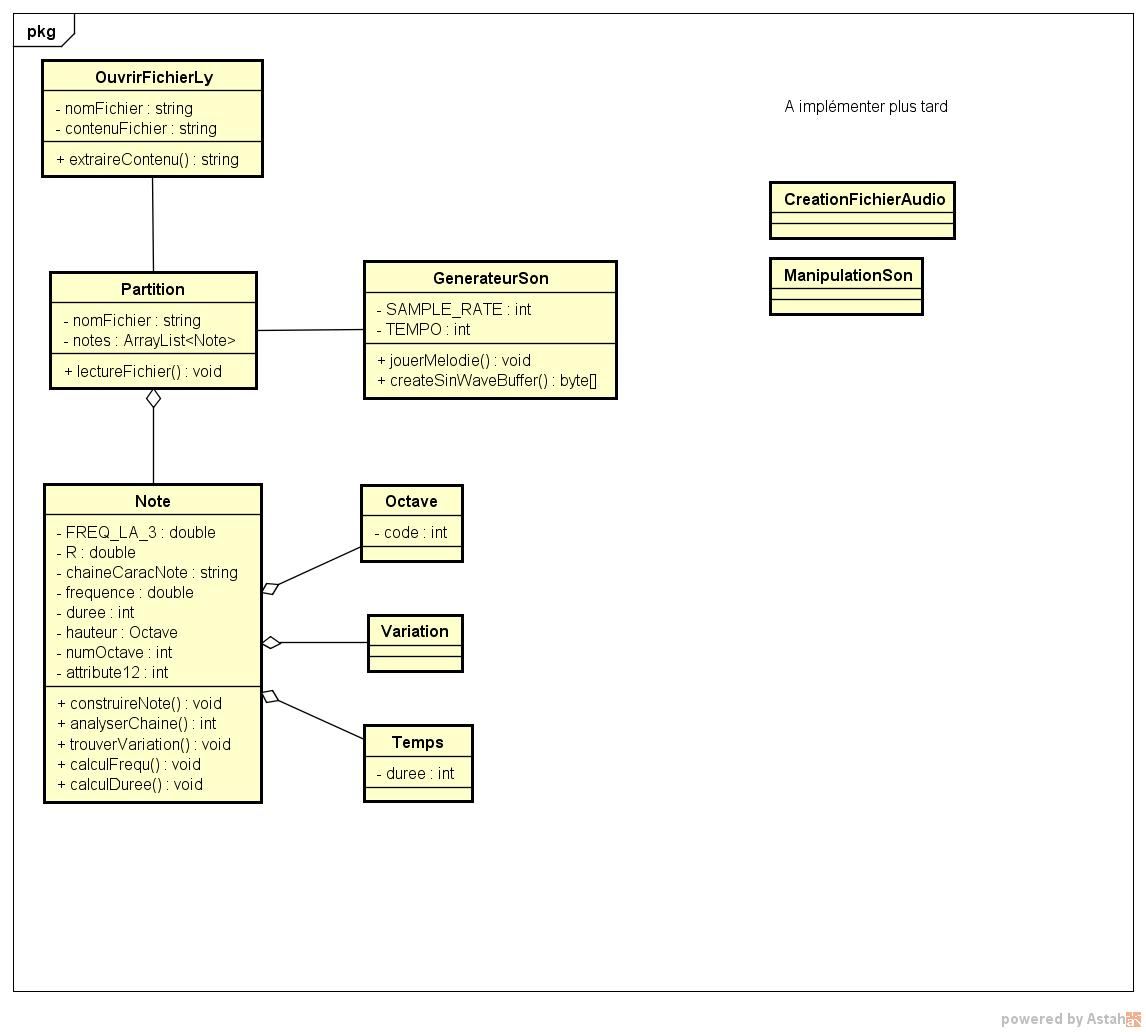
\includegraphics[scale=0.4]{Class_Diagram_MusicalSynth.jpg}
\captionof{figure}{Diagramme de classe première version}
\label{fig1}
\subsection{Classe Partition}

Le but de cette classe est de décrire la structure de partition.

Attributs :
\begin{itemize}
\item nom du fichier contenant le morceau
\item ArrayList de notes contenant la liste des notes à jouer dans l'ordre chronologique
\end{itemize}

Constructeur :
Cette méthode possède un constructeur prenant en paramètre le nom du fichier, qui sera mis dans les attributs.
Il lance ensuite la lecture du fichier, en appelant la méthode correspondante.

Accesseurs :
\begin{itemize}
\item getNotes() permet de récupérer l'ArrayList des notes.
\end{itemize}


Méthodes:
\begin{itemize}
\item lectureFichier() initialise la structure OuvrirFichierLy, puis récupère la chaîne de caractère qui a été lue dans le fichier, elle la sépare ensuite en fonction des espaces (appel de la méthode split), puis lance la construction des notes pour enfin les ajouter à l'ArrayList en attribut.
\end{itemize}

\subsection{Classe Notes}

Le but de cette classe est de construire caractériser une note, c'est à dire de calculer sa fréquence et sa durée en ms à partir de la chaîne contenue dans le fichier texte qui la décris.
Attributs :
\begin{itemize}
\item Fréquence de la note La (octave 3) a partir de laquelle toutes les autres notes sont calculées
\item R, le coefficient de la gamme pythagoricienne, multiplier la fréquence d'une note par cette constante la fait monter d'un demi ton, la diviser par la même constante la fait descendre. Sa valeur exacte est racine douzième de 2, on prends ici une valeur approchée.
\item La chaîne de caractère caractéristique de la note (cf notation Lilypond)
\item La fréquence de la note (en Hz)
\item La durée de la note (en ms)
\item La hauteur (do, ré, mi, mi\# etc...)
\item Le numéro de son octave (3 de base)
\item La variation (bémol, dièse ou neutre)
\end{itemize}

Constructeur :
Le constructeur mets la chaîne en paramètre dans les attributs puis initialise la construction de la note qui se déroule en 3 étapes: interprétation de la chaîne de caractère, calcul de la fréquence, et calcul de la durée.

Accesseurs :
On peut récupérer dans la structure: la fréquence, la durée et sa hauteur.

Méthodes :
\begin{itemize}
\item construireNote() appel successivement analyserChaine(), calculFrequ() (si la note n'est pas un silence) et calculDuree().
\item analyserChaine() va tout d'abord regarder la première lettre (= note en notation anglaise, de a à g, avec c = DO, d = RE etc...), si c'est un n, la fonction s'arrête en construisant un silence (frequence de 1, hauteur = NONE...) sinon, calcul du numéro de la note (voir enum Octave), appel de la fonction pour trouver la variation (voir trouverVariation()), modification de numNote si nécessaire enfin modification du numéro de l'octave si nécessaire.
\item trouverVariation() retire la première lettre de la chaine (qui correspond à la note qui a déjà été lue) puis recherche dedans les marqueurs des variations ('d' et 'is' pour le dièse, 'b' et 'es' pour le bémol)
\item calculFrequ(), prend d'abord comme fréquence de base celle du La3, puis la ramène à la bonne octave en multipliant ou divisant par un multiple de 2, puis multiplie par R le nombre de fois nécessaire pour arriver à la bonne fréquence.
\item calculDuree(), détecte le numéro à la fin de la chaine correspondant à la durée de la note.
\end{itemize}

\subsection{Classe GenerateurSon}

Attributs :
\begin{itemize}
\item L'échantillonage (nombre d'évalutaion de la valeur de l'onde sur un temps donné)
\item Le tempo (nombre de noires par minutes)
\end{itemize}

Méthodes :
\begin{itemize}
\item jouerMelodie(Partition part) initialise les structure de l'API java.Sound, puis parcours le tableau de notes de la partition en paramètre de la partition pour générer l'onde correspondante et la jouer sur la sortie standard, enfin, la méthode ferme le flux de sortie.
\item createSinWaveBuffer(double freq, int ms) crée un tableau de byte qui caractérise l'onde de fréquence passée en paramètre.
\end{itemize}


\subsection{OuvrirFichierLy}

Attributs :
\begin{itemize}
\item Nom du fichier contenant la description du morceau
\item Chaîne de caractère lue dans le fichier
\end{itemize}


Constructeur : 
\begin{itemize}
\item met le nom de fichier passé en paramètre dans les attributs, appel la fonction pour extraire le contenu du fichier.
\end{itemize}


Accesseurs :
\begin{itemize}
\item getContenu() permet de récupérer ce qui a été lu dans le fichier.
\end{itemize}

Méthodes :
\begin{itemize}
\item extraireContenu() permet de lire le fichier texte et de stocker le résultat dans l'attribut coresspondant.
\end{itemize}

\section{Perspectives pour la suite}

Pendant nos recherches, puis parallèlement à la rédaction de cette première version du code, nous avons également commencé à réfléchir à la façon de traiter la polyphonie avec cette application. Nous avons eu l'idée d'utiliser des Threads afin de traiter plusieurs tâches et donc lire plusieurs voix à la fois. La question que nous avons dû nous poser était la suivante : les Threads permettent-ils une lecture synchronisée des différentes voix ? Nous avons alors effectué quelques tests, et nous en avons déduits que nous pouvions totalement utiliser les Threads pour de la polyphonie. Nous adapterons notre code plus tard, il ne s'agit pas d'une fonctionnalité requise pour notre première version, il s'agissait plutôt de savoir si nous devions faire d'autres recherches ou si nous allions pouvoir utiliser les Threads dans le code.

\chapter{Itération 2}

%--------------------------------------------------------------------------------
%\chapter*{Conclusion}
%\addcontentsline{toc}{chapter}{\numberline{}Conclusion}
%\markboth{Conclusion}{}

%\label{sec:conclusion}

%--------------------------------------------------------------------------------
%exemple de bibliographie
\begin{thebibliography}{99}
\item \url{http://www.commentcamarche.net/forum/affich-590149-lire-un-fichier-texte-en-java}
\item \url{http://stackoverflow.com/questions/8632104/sine-wave-sound-generator-in-java}
\label{sec:biblio}
\end{thebibliography}


%--------------------------------------------------------------------------------
%si on donne des annexes :
\appendix
\addcontentsline{toc}{part}{\numberline{}Annexes}

%--------------------------------------------------------------------------------

\chapter{Liens utiles\label{sec:liens_utiles}}
Voici une petite liste d'url intéressantes au sujet de ce projet :

\begin{itemize}
\item \url{www.polytech.univ-tours.fr}
\item Syntaxe Lilypond : \url{http://lilypond.org/text-input.html}
\item Documentation complète Lilypond : \url{http://lilypond.org/doc/v2.18/Documentation/learning.pdf}
\item \url{http://docs.oracle.com/javase/7/docs/technotes/guides/sound/programmer_guide/contents.html}
\item \url{https://www.openal.org/documentation/openal-1.1-specification.pdf}
\item \url{http://www.fmod.org/documentation/}
\end{itemize}
%--------------------------------------------------------------------------------
%index : attention, le fichier dindex .ind doit avoir le même nom que le fichier .tex
%\printindex

%--------------------------------------------------------------------------------
%page du dos de couverture :

\resume{A compléter}

\motcles{???, ????, ?????, ?????????, ??, ????}

\abstract{To complete later}

\keywords{???, ????, ?????, ?????????, ??, ????}


\makedernierepage


\end{document}
%%FIN du fichier